\documentclass[final,hyperref={pdfpagelabels=false}]{beamer}
\mode<presentation>
  {
  \usetheme{Dreuw}
  \usefonttheme[mathonly]{serif}
  }
  \usepackage{times}
  \usepackage{amsmath,amsthm, amssymb, latexsym}
  \usepackage[english]{babel}
  \usepackage[latin1]{inputenc}
  \usepackage[orientation=landscape,size=a0,scale=1.4,debug]{beamerposter}

  \newcommand{\R}{\mathbb{R}}
  \newcommand{\D}{\mathbb{D}}
  \newcommand{\F}{\mathbb{F}}
  \newcommand{\Z}{\mathbb{Z}}
  \newcommand{\Zeq}{\mathbb{Z}_{\geq 0}}
  \newcommand{\Zg}{\mathbb{Z}_{>0}}
  \newcommand{\Req}{\mathbb{R}_{\geq 0}}
  \newcommand{\Rg}{\mathbb{R}_{>0}}
  \newcommand{\N}{\mathbb{N}}
  \newcommand{\E}{\mathbb{E}}
  \newcommand{\Q}{\mathbb{Q}}
  \newcommand{\Ha}{\mathbb{H}}
  \newcommand{\C}{\mathbb{C}}
  \newcommand{\lpnorm}[2]{\left|\left|{#1}\right|\right|_{L^{#2}}}
  \DeclareMathOperator{\ima}{im}
  \DeclareMathOperator{\spn}{span}
  \DeclareMathOperator{\rank}{rank}
  \DeclareMathOperator{\real}{Re}
  \DeclareMathOperator{\imag}{Im}
  \DeclareMathOperator{\diver}{div}
  \DeclareMathOperator{\curl}{curl}
  \DeclareMathOperator{\id}{id}
  \DeclareMathOperator{\inter}{int}
  \DeclareMathOperator{\Dr}{Dr}
  \DeclareMathOperator{\Jac}{Jac}
  \DeclareMathOperator{\Cov}{Cov}
  \DeclareMathOperator{\Var}{Var}
  \DeclareMathOperator{\res}{res}

  %%%%%%%%%%%%%%%%%%%%%%%%%%%%%%%%%%%%%%%%%%%%%%%%%%%%%%%%%%%%%%%%%%%%%%%%%%%%%%%%%5
  \graphicspath{{figures/}}
  \title[fBM Estimation Under Noise]{Estimating Fractional Brownian Motion With Noise}
  \author[Chen & Jia & Monier & Shen]{David Chen, Wangdong Jia, Bryce Monier, Shiyang Shen}
  \institute[Columbia University]{Columbia Math Undergraduate Summer Research Program}
  \date{Jul. 31th, 2007}


  %%%%%%%%%%%%%%%%%%%%%%%%%%%%%%%%%%%%%%%%%%%%%%%%%%%%%%%%%%%%%%%%%%%%%%%%%%%%%%%%%5
  \begin{document}
  \begin{frame}{} 
    \vfill
    \begin{columns}[t]
      \begin{column}{0.28\linewidth}
        \begin{block}{Introduction}
          Suppose we have some unknown fBM with stochastic volatility, \(X_t\), and some process with added noise that we are able to observe: \(Y_t = X_t + \rho Z_t\).  We would like to be able to extract the signal from the noise, and to somehow estimate both \(H\) and \(\sigma\). To do so, we will consider weighted averages of \(Y_t\) at different time-points to eliminate the noise. Estimators of \(H\) and the integrated volatility have been previously shown for fBM without noise [2] and without stochastic volatility [3]; the main result of this project is to combine both generalizations.
        % Fractional Brownian Motion (fBM) is an important generalization of Brownian Motion parameterized by the Hurst index. The Hurst index is a real-valued number \(H \in (0,1)\) that characterizes continuous processes that are ``rougher'' (when \(H < 1/2\)) or ``smoother'' (when \(H > 1/2\)) than standard Brownian motion, which is exactly defined by fBM with \(H = 1/2\). In this presentation, we show how one may construct an estimator for an unknown Hurst index \(H\) given a single realized path of an fBM whose values are only observed with measurement noise. The main tool to develop this estimator is a theorem considering what quadratic variation-type functionals of these processes would converge to. The proof of this theorem is the main result of this REU project and adapts previously seen techniques such as pre-averaging, truncation and discretization to our current setting. Our results also allow us to derive estimators for \(H\) in the presence of stochastic volatility.
        \end{block}
        \begin{block}{Background and Setup}
          \begin{itemize}
            \item The Riemann-Liouville fractional Brownian motion with Hurst Index \(H\) is the process given by the stochastic integral
              \[
                B^H_t := \int_0^t (t-s)^{H - \frac{1}{2}} \ dB_s.
              \]
            \item Measurement noise will be considered as random normal variables with variance \(\rho^2\).
            \item We consider the following process:
              \[
                Y_t = X_0 + \int_0^t b_sds + K^{-\frac{1}{2}}_HB^H_t + \rho Z_t,
              \]
              where \(\int_0^t b_sds\) is some drift process, \(K^{-\frac{1}{2}}_H\) is a normalizing constant, and \((Z_t)_{t \geq 0}\) are i.i.d. \(N(0,1)\) variables.
          \end{itemize}
        \end{block}
        \begin{block}{Pre-Averaging}
          We attempt to remove the error from the process by considering weighted averages of the increments of \(Y_t\) to try and smooth out the random noise. The variation from these \textit{pre-averages} are then used to construct estimators for \(H\) and \(\int_0^T \sigma^2 ds\). Formally, for \(g: [0,1] \rightarrow \R\), some constant \(\theta\), and some stochastic process \(W_t\), put
          \begin{gather*}
            k_n = \frac{n^\kappa}{\theta}, \ g^n_j = g\left( \frac{j}{k_n} \right) \\
            \overline{W}(g)^n_i = \sum_{j=1}^{k_n-1}g^n_j\left( W_{\frac{i+j-1}{n}} - W_{\frac{i+j-2}{n}} \right) = \sum_{j=1}^{k_n-1}g^n_j\Delta_{i+j-1}^n W \\
            \widehat{W}(g)^n_i = \sum_{j=1}^{k_n}\left(g^n_j - g^n_{j-1}\right)^2\left(\Delta_{i+j-1}^n W\right)^2 = \sum_{j=1}^{k_n}\left(\Delta g^n_j\right)^2\left(\Delta_{i+j-1}^n W\right)^2.
          \end{gather*}
        \end{block}
      \end{column}

      \begin{column}{0.4\linewidth}
        \begin{block}{Main Theorem}
          Given some fBM with measurement error,
          \begin{equation*}
            Y_t = X_t + \rho Z_t
          \end{equation*}
          if we have the following conditions,
          \begin{enumerate}
            \item \(f: \R^L \rightarrow \R\) is \(C^2\) with all partial derivatives up to order 2 of at most polynomial growth.
            \item \(g: [0,1] \rightarrow \R\) is \(C^2\).
            \item \(b, \sigma\) are of size 1 (that is, \(||b_s||_{L_p}, ||\sigma_s||_{L_p}\) are bounded) and adapted.
            \item \(\sigma\) is \(L^2\)-continuous.
            \item \(\kappa \in \left(\frac{2H}{2H+1}, 1\right)\).
          \end{enumerate}
          then we get the following convergence:
          \begin{equation*}
            V(g)^{n,f}_T(Y) = \frac{1}{n}\sum_{i=1}^{\left\lfloor nT \right\rfloor}f\left( \frac{\overline{Y}(g)^n_i}{\left( k_n/n \right)^H}, \frac{\widehat{Y}(g)^n_i}{\left( k_n/n \right)^{2H}} \right) \overset{\mathbb{P}}{\rightarrow} \int_0^T \mu_f\left( \sigma_s^2\eta^H\left( g \right), \Theta^2\rho^2 \int_0^1g'(r)^2dr \right)ds
          \end{equation*}
          where
          \begin{gather*}
            \mu_f(v_1, v_2) = \E\left[ f\left(v_1Z_2 + v_2Z_2, 2v_2\right) \right], \ Z_1, Z_2 \sim N(0, 1) \text{ i.i.d.} \\
            \Theta =
            \begin{cases}
              0 & \kappa \neq \frac{2H}{2H+1} \\
              \theta &  \kappa = \frac{2H}{2H+1}
            \end{cases} \\
            \eta^H(g) = 2H\int_0^1g(x)\left(g(1)(1-x)^{2H-1} + \int_x^1(y-x)^{2H-1}g'(y)dy\right)dx
          \end{gather*}
        \end{block}

        \begin{block}{Sketch of the Proof}
          We make a series of adjustments to \(V(g)^{n,f}_T(Y)\) to get closer to our final result. We first remove the drift: if \(U_t = K_H^{-\frac{1}{2}}B^H_t + \rho Z_t\),
          \begin{equation*}
            \lim_{n \rightarrow \infty} \E\left[ \left| V(g)^{n,f}_T(Y) - V(g)^{n,f}_T(U) \right| \right] = 0.
          \end{equation*}
          We show also that one can truncate the the domain of integration to within \(\epsilon\) of where we first begin averaging, i.e. \(\frac{i}{n} - \epsilon\) while making only an error bounded by \(\epsilon\).
          % Next, we \textit{truncate} the domain of integration in the stochastic integral to \(\epsilon\) of where we begin averaging; a truncated increment of fBM is defined as
          % \begin{equation*}
          %   \Delta_{i+j-1}^{n,\epsilon} B^H_t =  \int_{\frac{i}{n}-\epsilon}^{\frac{i+j-1}{n}} \left[ \left( \frac{i+j-1}{n} -s \right)^{H - \frac{1}{2}} - \left( \frac{i+j-1}{n} -s \right)^{H - \frac{1}{2}} \right]\sigma_s dB_s.
          % \end{equation*}
          % With this, we get
          % \begin{equation*}
          %   \limsup_{n \rightarrow \infty} \E \left[ \left| V(g)^{n,f}_T(U) - \frac{1}{n}\sum_{i=\left\lfloor n\epsilon \right\rfloor + 1}^{\left\lfloor nT \right\rfloor} f\left( \frac{\overline{U}(g)^{n,\epsilon}_i}{(k_n/n)^H}, \frac{\widehat{U}(g)^{n,\epsilon}_i}{(k_n/n)^{2H}} \right) \right| \right] < C\epsilon
          % \end{equation*}
          We now \textit{discretize} the volatility by showing that
          \begin{align*}
            \phantom{}
            \begin{aligned}
      &\lim_{\epsilon \rightarrow 0}\lim_{n \rightarrow \infty}\E \left[ \left| \frac{1}{n}\sum_{i=\left\lfloor n\epsilon \right\rfloor + 1}^{\left\lfloor nT \right\rfloor} \left[ V(g)^{n,f}_T(Y) -  f\left( \frac{\sigma_{\frac{i}{n}-\epsilon}\overline{B^H}(g)^{n,\epsilon}_i + \rho\overline{Z}(g)^n_i}{(k_n/n)^{H}}, \frac{\rho^2\widehat{Z}(g)^n_i}{(k_n/n)^{2H}}\right) \right] \right| \right] = 0
            \end{aligned}
          \end{align*}
          We now center to the conditional expectation:
          \begin{align*}
            \phantom{}
    &\begin{aligned}
      &\frac{1}{n}\sum_{i = \left\lfloor n\epsilon \right\rfloor + 1}^{\left\lfloor nT \right\rfloor} \left[ \vphantom{\E \left[ f\left( \frac{\sigma_{\frac{i}{n}-\epsilon}\overline{B^H}(g)^{n,\epsilon}_i + \rho\overline{Z}(g)^n_i}{(k_n/n)^{2H}}, \frac{\rho^2\widehat{Z}(g)^n_i}{(k_n/n)^H}\right) \right] } f\left( \frac{\sigma_{\frac{i}{n}-\epsilon}\overline{B^H}(g)^{n,\epsilon}_i + \rho\overline{Z}(g)^n_i}{(k_n/n)^{2H}}, \frac{\rho^2\widehat{Z}(g)^n_i}{(k_n/n)^H}\right) \right. \\ &\hspace*{2.1cm} - \left. \E\left[ f\left( \frac{\sigma_{\frac{i}{n}-\epsilon}\overline{B^H}(g)^{n,\epsilon}_i + \rho\overline{Z}(g)^n_i}{(k_n/n)^{H}}, \frac{\rho^2\widehat{Z}(g)^n_i}{(k_n/n)^{2H}}\right) \big| \mathcal{F}_{\frac{i-1}{n}} \right] \vphantom{\frac{1}{n}\sum_{i = \left\lfloor n\epsilon \right\rfloor + 1}^{\left\lfloor nT \right\rfloor}} \right] \overset{\mathbb{P}}{\rightarrow} 0
    \end{aligned}
          \end{align*}
          Once we compute the expectation and take limits (\(n \rightarrow \infty\), \(\epsilon \rightarrow 0\)), we arrive at what we wanted.
        \end{block}
      \end{column}

      \begin{column}{0.28\linewidth}
        % \begin{block}{Sketch of the Proof (Cont.)}
        % \end{block}
        \begin{block}{Estimating \(H\)}
          Changing the freqency of the averaging allows us to create an estimator for \(H\); consider taking \(f(x, y) = x^2 - \frac{1}{2}y\) and a suitable \(\kappa\) such that \(\Theta = 0\), such that 
          \begin{align*}
            V(g)^{n,f}_T(Y), \ V(g)^{\frac{n}{2},f}_T(Y) &= \frac{2}{n}\sum_{i=1}^{\left\lfloor nT/2 \right\rfloor} \left(\frac{\overline{Y}(g)^{n/2}_i}{(2k_n/n)^H}\right)^2
          \end{align*}
          both converge in probability to \( \int_0^T \sigma^2\eta^H(g) ds\), so
          \[
            \frac{1}{2(1 - \kappa)} \log_2\left(\frac{\widetilde{V}(g)^{\frac{n}{2},f}_T(Y)}{\widetilde{V}(g)^{n,f}_T(Y)}\right) \overset{\mathbb{P}}{\rightarrow} H.
          \]
          where \(\widetilde{V}(g)^{n,f}_T(Y)\) is simply \(V(g)^{n,f}_T(Y)\) without the normalizing factor.
          Furthermore, we can estimate the integrated volatility:
          \[
            \frac{V(g)^{n,f}_T(Y)}{\eta^{\hat{H}_n}(g)} \rightarrow \int_0^T\sigma^2_sds.
          \]
        \end{block}
        \begin{block}{In Practice}
          % To compute such an estimator, one may take \(\kappa = \frac{2}{3}\) in order to guarantee that \(\Theta\) vanishes, in which case we can consistently (given large \(n\)) estimate \(H\) and \(\int_0^T \sigma_s^2ds\).
          Estimating simulated datasets with \(n = 10^5\) and random Hurst indices, the following is \(\hat{H}_n\) plotted against \(H\). Plotted line is just the identity, which we expect our estimators to converge to.

          \begin{center}
            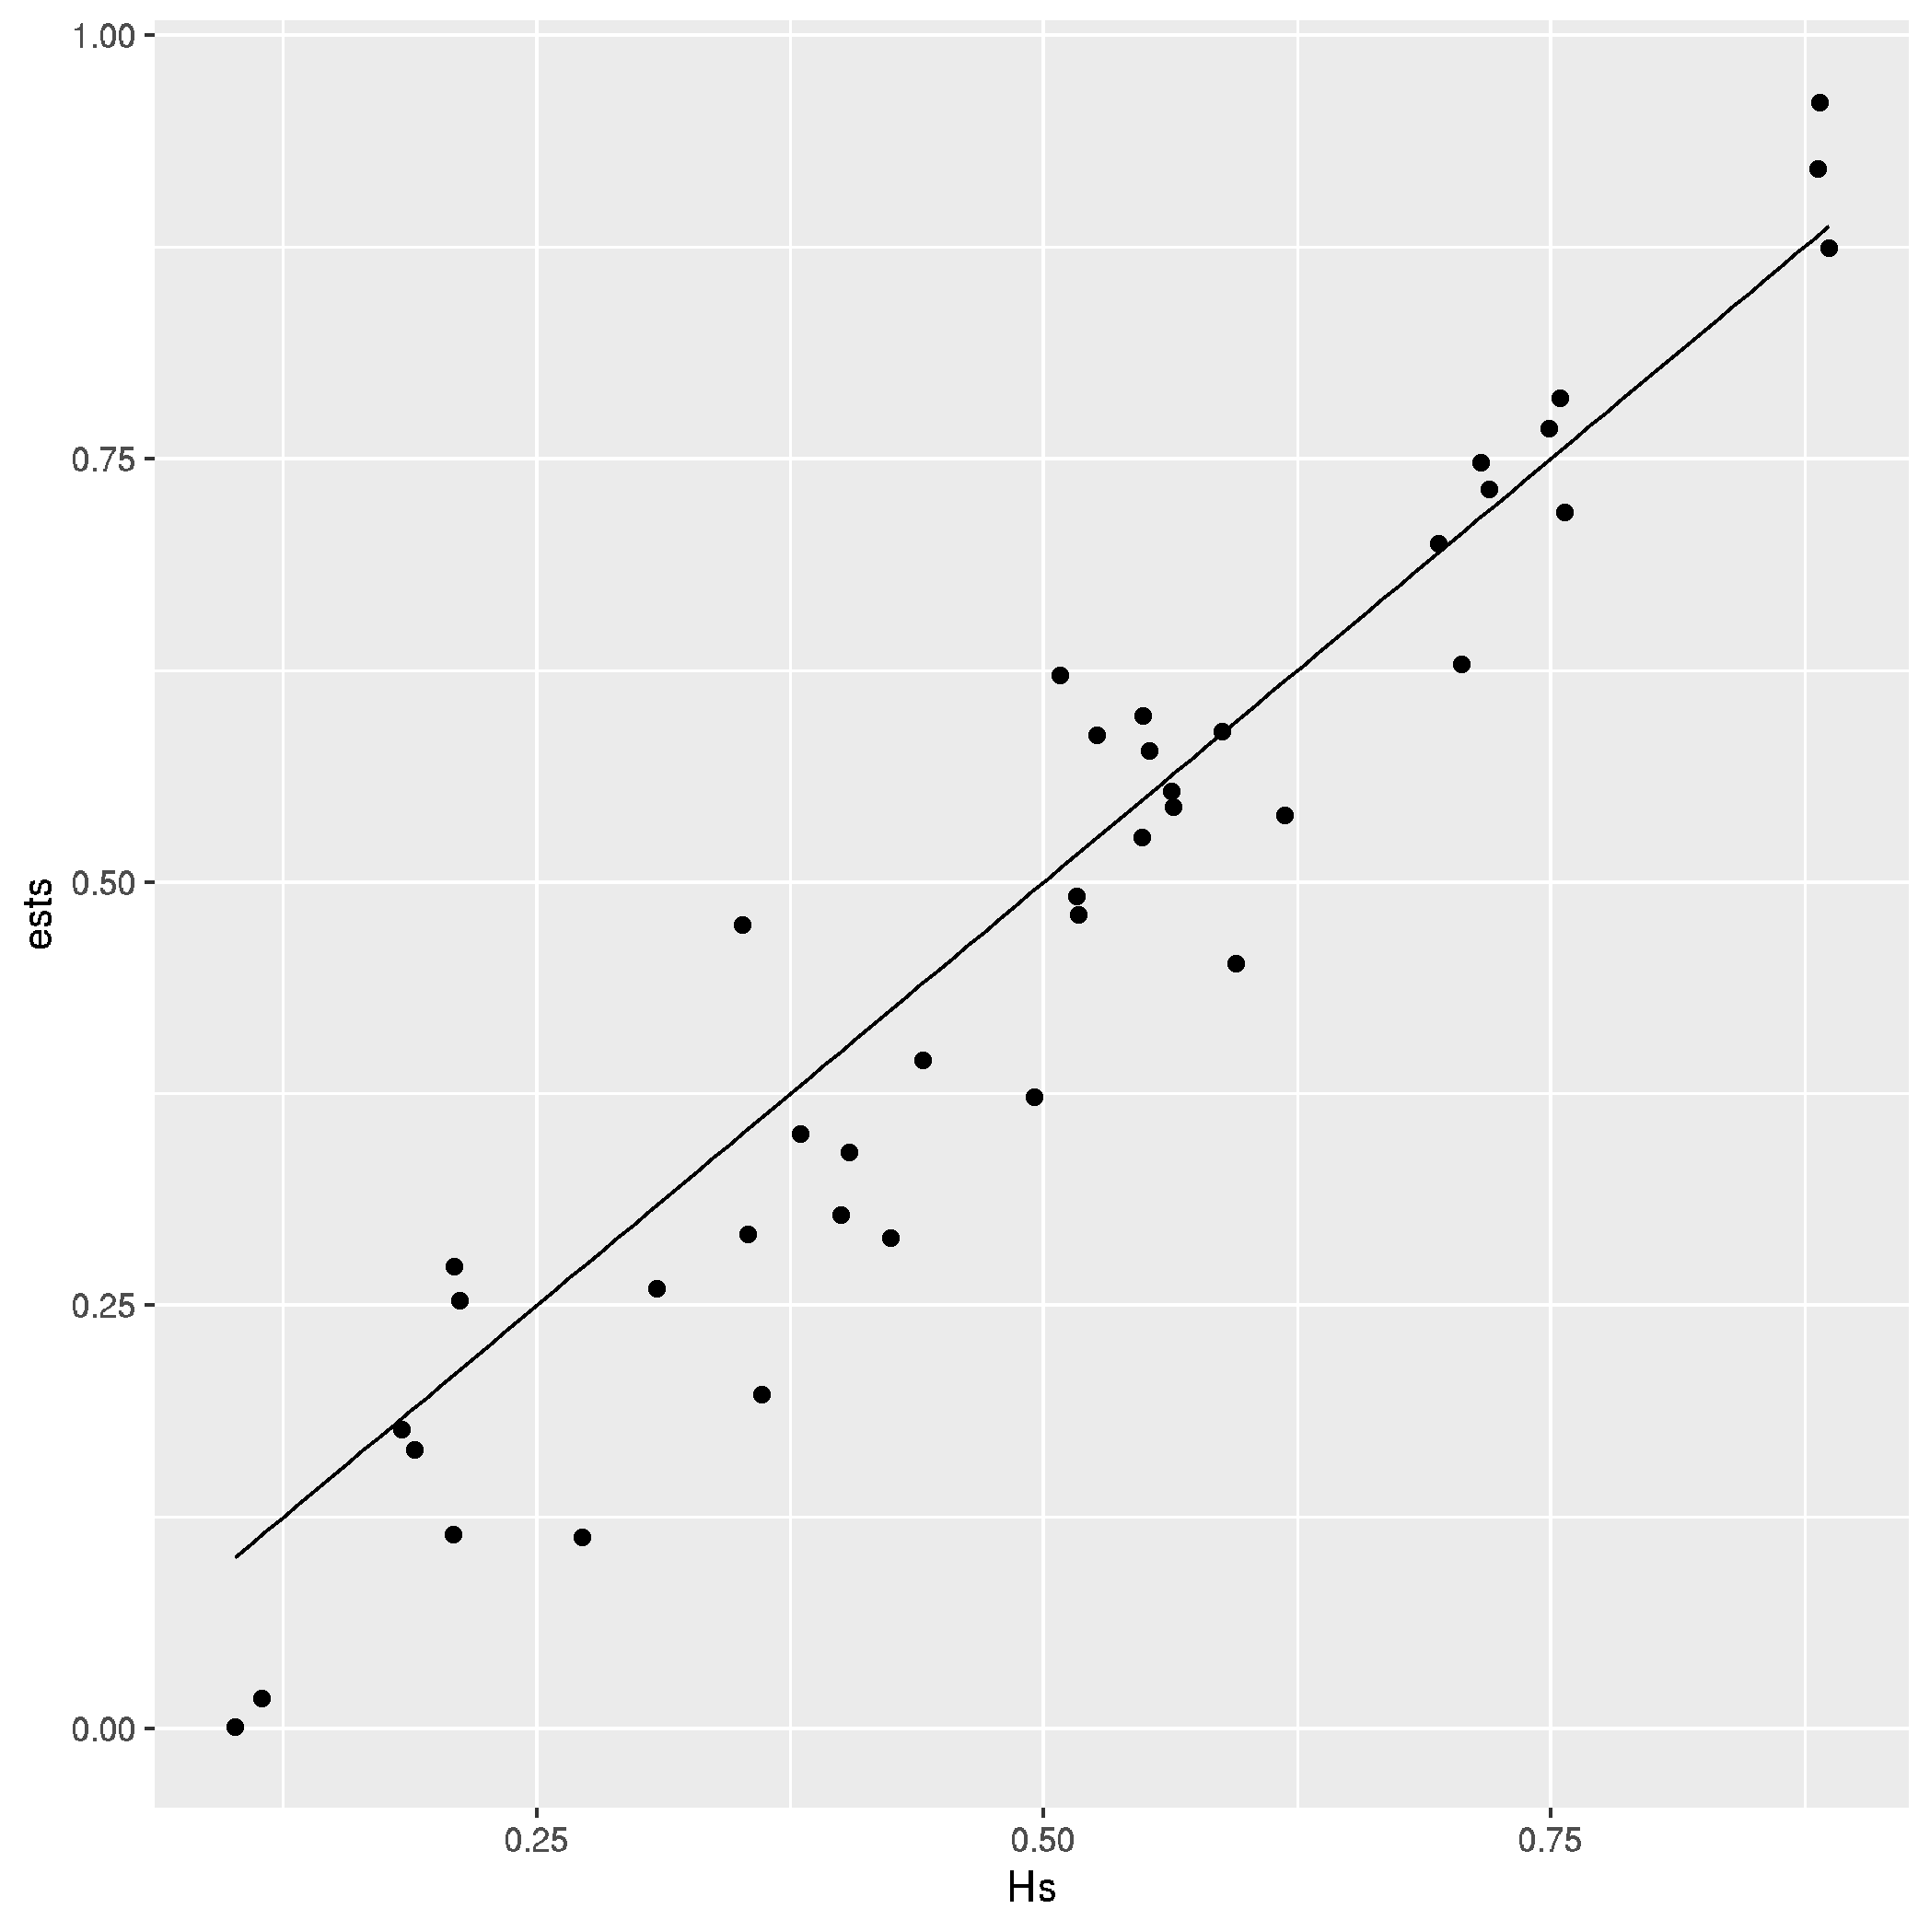
\includegraphics[width=15cm]{./hests.png}
          \end{center}
          Consistent estimations of the volatility, for which convergence is slow, is an ongoing effort; related code may be found at [4].
        \end{block}
        \begin{block}{Acknowledgements and References}
          {\footnotesize
            First, we would like to thank Dr. Carsten Chong for his guidance and support in this project before, during, and after the research, as well as the Columbia Mathematics Undergraduate Summer Research Program.
          }{\tiny
          \begin{enumerate}
            \item Jacod, J., Li, Y., Mykland, P. A., Podolskij, M., Vetter, M.: Microstructure noise in the continuous case: the pre-averaging approach. Stochastic Process. Appl. 119 (2009), no. 7, 2249-2276.
            \item Corcuera, J. M., Hedevang, E., Pakkanen, M. S., Podolskij, M.: Asymptotic theory for Brownian semi-stationary processes with application to turbulence. Stochastic Process. Appl. 123 (2013), no. 7, 2552-2574.
            \item Gloter, A, and Hoffmann, M.: Estimation of the Hurst parameter from discrete noisy data. Ann. Statist. 35 (2007), no. 5, 1947-1974.
            \item https://github.com/DaisiesForAMouse/REU-Writeup
          \end{enumerate}
        }
        \end{block}
      \end{column}
    \end{columns}
  \end{frame}
\end{document}

